\documentclass[english,notitlepage,reprint]{revtex4-1}  % defines the basic parameters of the document

% if you want a single-column, remove reprint

% allows special characters (including æøå)
\usepackage[utf8]{inputenc}
\usepackage[english]{babel}

%% note that you may need to download some of these packages manually, it depends on your setup.
%% I recommend downloading TeXMaker, because it includes a large library of the most common packages.

\usepackage{physics,amssymb}  % mathematical symbols (physics imports amsmath)
\usepackage{graphicx}         % include graphics such as plots
\usepackage{xcolor}           % set colors
\usepackage{hyperref}         % automagic cross-referencing (this is GODLIKE)
\usepackage{tikz}             % draw figures manually
\usepackage{listings}         % display code
\usepackage{subfigure}        % imports a lot of cool and useful figure commands
\usepackage{lipsum}

\usepackage{lmodern}

% (2) specify encoding
\usepackage[T1]{fontenc}
\usepackage{textcomp}
%\usepackage{unicode-math}
\usepackage{float}
\usepackage{balance}

% defines the color of hyperref objects
% Blending two colors:  blue!80!black  =  80% blue and 20% black
\hypersetup{ % this is just my personal choice, feel free to change things
    colorlinks,
    linkcolor={red!50!black},
    citecolor={blue!50!black},
    urlcolor={blue!80!black}}

%% Defines the style of the programming listing
%% This is actually my personal template, go ahead and change stuff if you want
\lstset{ %
	inputpath=,
	backgroundcolor=\color{white!88!black},
	basicstyle={\ttfamily\scriptsize},
	commentstyle=\color{magenta},
	language=Python,
	morekeywords={True,False},
	tabsize=4,
	stringstyle=\color{green!55!black},
	frame=single,
	keywordstyle=\color{blue},
	showstringspaces=false,
	columns=fullflexible,
	keepspaces=true}

\lstset{literate=
  {á}{{\'a}}1 {é}{{\'e}}1 {í}{{\'i}}1 {ó}{{\'o}}1 {ú}{{\'u}}1
  {Á}{{\'A}}1 {É}{{\'E}}1 {Í}{{\'I}}1 {Ó}{{\'O}}1 {Ú}{{\'U}}1
  {à}{{\`a}}1 {è}{{\`e}}1 {ì}{{\`i}}1 {ò}{{\`o}}1 {ù}{{\`u}}1
  {À}{{\`A}}1 {È}{{\'E}}1 {Ì}{{\`I}}1 {Ò}{{\`O}}1 {Ù}{{\`U}}1
  {ä}{{\"a}}1 {ë}{{\"e}}1 {ï}{{\"i}}1 {ö}{{\"o}}1 {ü}{{\"u}}1
  {Ä}{{\"A}}1 {Ë}{{\"E}}1 {Ï}{{\"I}}1 {Ö}{{\"O}}1 {Ü}{{\"U}}1
  {â}{{\^a}}1 {ê}{{\^e}}1 {î}{{\^i}}1 {ô}{{\^o}}1 {û}{{\^u}}1
  {Â}{{\^A}}1 {Ê}{{\^E}}1 {Î}{{\^I}}1 {Ô}{{\^O}}1 {Û}{{\^U}}1
  {œ}{{\oe}}1 {Œ}{{\OE}}1 {æ}{{\ae}}1 {Æ}{{\AE}}1 {ß}{{\ss}}1
  {ű}{{\H{u}}}1 {Ű}{{\H{U}}}1 {ő}{{\H{o}}}1 {Ő}{{\H{O}}}1
  {ç}{{\c c}}1 {Ç}{{\c C}}1 {ø}{{\o}}1 {å}{{\r a}}1 {Å}{{\r A}}1
  {€}{{\euro}}1 {£}{{\pounds}}1 {«}{{\guillemotleft}}1
  {»}{{\guillemotright}}1 {ñ}{{\~n}}1 {Ñ}{{\~N}}1 {¿}{{?`}}1
}

%% USEFUL LINKS:
%%
%%   UiO LaTeX guides:        https://www.mn.uio.no/ifi/tjenester/it/hjelp/latex/
%%   mathematics:             https://en.wikibooks.org/wiki/LaTeX/Mathematics

%%   PHYSICS !                https://mirror.hmc.edu/ctan/macros/latex/contrib/physics/physics.pdf

%%   the basics of Tikz:       https://en.wikibooks.org/wiki/LaTeX/PGF/TikZ
%%   all the colors!:          https://en.wikibooks.org/wiki/LaTeX/Colors
%%   how to draw tables:       https://en.wikibooks.org/wiki/LaTeX/Tables
%%   code listing styles:      https://en.wikibooks.org/wiki/LaTeX/Source_Code_Listings
%%   \includegraphics          https://en.wikibooks.org/wiki/LaTeX/Importing_Graphics
%%   learn more about figures  https://en.wikibooks.org/wiki/LaTeX/Floats,_Figures_and_Captions
%%   automagic bibliography:   https://en.wikibooks.org/wiki/LaTeX/Bibliography_Management  (this one is kinda difficult the first time)
%%   REVTeX Guide:             http://www.physics.csbsju.edu/370/papers/Journal_Style_Manuals/auguide4-1.pdf
%%
%%   (this document is of class "revtex4-1", the REVTeX Guide explains how the class works)


%% CREATING THE .pdf FILE USING LINUX IN THE TERMINAL
%%
%% [terminal]$ pdflatex template.tex
%%
%% Run the command twice, always.
%% If you want to use \footnote, you need to run these commands (IN THIS SPECIFIC ORDER)
%%
%% [terminal]$ pdflatex template.tex
%% [terminal]$ bibtex template
%% [terminal]$ pdflatex template.tex
%% [terminal]$ pdflatex template.tex
%%
%% Don't ask me why, I don't know.

\usepackage{thmtools}
\DeclareMathOperator{\nullspace}{Nul}
\DeclareMathOperator{\collspace}{Col}
\DeclareMathOperator{\rref}{Rref}
%%\DeclareMathOperator{\dim}{Dim}

 % "meq": must be equal
\newcommand{\meq}{\overset{!}{=}}

\newcommand{\R}{\mathbb{R}}
\newcommand*\Heq{\ensuremath{\overset{\kern2pt L'H}{=}}}
\usepackage{bm}
\newcommand{\uveci}{{\bm{\hat{\textnormal{\bfseries\i}}}}}
\newcommand{\uvecj}{{\bm{\hat{\textnormal{\bfseries\j}}}}}
\DeclareRobustCommand{\uvec}[1]{{%
  \ifcsname uvec#1\endcsname
     \csname uvec#1\endcsname
   \else
    \bm{\hat{\mathbf{#1}}}%
   \fi
}}
\usepackage{siunitx}

\makeatletter
\newcommand*{\balancecolsandclearpage}{%
  \close@column@grid
  \cleardoublepage
  \twocolumngrid
}
\makeatother

\newcounter{subproject}
\renewcommand{\thesubproject}{\alph{subproject}}
\newenvironment{subproj}{
\begin{description}
	\item[\refstepcounter{subproject}(\thesubproject)]
}{\end{description}}


\begin{document}
\title{Numerical integration using the Thomas algorithm}   % self-explanatory
\author{Anders P. Åsbø}               % self-explanatory
\date{\today}
\noaffiliation                            % ignore this

\begin{abstract}
The focus of this paper was the specific case of numerically integrating a linear, second order differential equation as a system of linear equations by deriving, and implementing the Thomas algorithm\citep{Datta2010}, as well as the precision and computational speed of the algorithm.

It proved to be a efficient, and sufficiently precise method for integrating a second order, linear differential equation. The specialized variant of the algorithm proved especially memory efficient. Both the general, and specialized Thomas algorithms are preferable for the specific usecase in this paper, as they used significantly less memory, and time than a general LU-decomposition solver.
\end{abstract}

\maketitle
\tableofcontents

\section{Introduction}\label{sec:1}
Numerical integration is an important cornerstone of computational physics, and as such it is important to understand its limits in terms of numerical precision and time spent computing. In this report I have looked at the specific case of numerically integrating a linear, second order differential equation as a system of linear equations, with the pretext of solving a one-dimensional variant of Poisson's equation. The focus of this paper will be on deriving, and implementing the Thomas algorithm\citep{Datta2010}, as well as the precision and computational speed of the algorithm.

All code for this report was written in Python 3.6, and the complete set of program files can be found at \url{https://github.com/FunkMarvel/CompPhys-Project-1}.

\section{Formalism}\label{sec:2}
\subsection{Underlying theory}\label{subsec:21}
If I have a charge distrobution \(\rho(\vec{r})\), as a function of the position \(\vec{r}\), Possion's equation gives the electrostatic potential \(\Phi\)
$$
	\nabla^{2}=-4\pi\rho(\vec{r})
$$
\citep{DepartmentofPhysics2019}. If I then assume both \(\rho(\vec{r})\), and \(\Phi\) to be spherically symetric, the equation can be simplified to
$$
	\frac{1}{r^{2}}\frac{d\Phi}{dr}r^{2}\frac{d\Phi}{dr}=-4\pi\rho(r),
$$
where \(r=|\vec{r}|\). Substituting \(\Phi(r)=\frac{1}{r}\phi(r)\) gives
$$
	\frac{d^{2}\phi}{dr^{2}}=-4\pi\rho(r),
$$
which, for simplicity, can be written as
$$
	-u''(x)=f(x),
$$
with \(u = \phi\), \(f=-4\pi\rho\), and \(x = r\)\citep{DepartmentofPhysics2019}.

Having arrived at a simple formulation of the initial problem, I can now discretize it using the second order differential approximation
$$
	-\frac{u(x+h)+u(x-h)-2u(x)}{h^{2}}=f(x).
$$
Since I will be opperating with a discreete set of variables \(x_{i}\in[0,1]\) where \(x_{i}=ih\) for \(i=1,2,3,...,N\), I can write the afformentioned approximation as
$$
	-\frac{u_{i+1}+u_{i-1}-2u_{i}}{h^{2}}=f_{i},
$$
where \(u_{i}=u(x_{i})\). The step-size is defined as \(h=\frac{x_{N}-x_{0}}{N}\), and I impose the Dirichlet boundary conditions \(u(0)=u(1)=0\)\citep{DepartmentofPhysics2019}.

\subsection{Deriving an algorithm for square, tridiagonal matricies}\label{subsec:22}

The discretized approximation obtained in \hyperref[subsec:21]{II.B} can be rearranged to
$$
	-1u_{i-1}+2u_{i}-1u_{i+1}=h^{2}f_{i},
$$
which describes a tridiagonal, \(N\cross N\)-matrix
$$
	A =
	\begin{bmatrix}
	2 & -1 & 0 & \dots & 0 \\
	-1 & 2 & -1 & \ddots &\vdots \\
	0 & -1 & 2 & -1 & \vdots \\
	\vdots & \ddots & \ddots & \ddots & \vdots \\
	\vdots & \dots & \dots & -1 & 2 \\
	\end{bmatrix},
$$
and with the unkowns in a vector
$$
	\vec{u} =
	\begin{bmatrix}
		u_{1} \\
		\vdots \\
		u_{N} \\
	\end{bmatrix},
$$
and the values of \(h^{2}f_{i} = g_{i}\) in a vector
$$
	\vec{g} =
	\begin{bmatrix}
		g_{1} \\
		\vdots \\
		g_{N} \\
	\end{bmatrix},
$$
I can express the integration problem as a matrix equation
$$
	A\vec{u}=\vec{g}.
$$

For a general matrix
$$
	A =
	\begin{bmatrix}
	d_{1} & a_{1} & 0 & \dots & \dots & 0 \\
	b_{1} & d_{2} & a_{2} & \ddots & \ddots &\vdots \\
	0 & b_{2} & d_{3} & a_{3} & \ddots & \vdots \\
	\vdots & \ddots & \ddots & \ddots & \ddots & \vdots \\
	\vdots & \ddots & \ddots & \ddots & \ddots & a_{N-1} \\
	0 & \dots &\dots & \dots & b_{N-1} & d_{N} \\
	\end{bmatrix}
$$
\citep{DepartmentofPhysics2019}. A way to solve the matrix equation is by Gaussian elimination. I start by subtracting row 1 multiplied by \(\frac{b_{1}}{d_{1}}\) from row 2, and continue by subtracting row 2 multiplied by \(\frac{b_{2}}{d_{2}}\) from row 3. This continues all the way down such that a general algorithm can be written as
\begin{equation}
	d_{i}^{*}=d_{i}-\frac{b_{i-1}a_{i-1}}{d_{i-1}^{*}}, \label{eq:1}
\end{equation}
with the condition that \(d^{*}_{1}=d_{1}\). The same pattern aplies to \(\vec{g}\), such that
\begin{equation}
	g_{i}^{*} = g_{i}-\frac{b_{i-1}g_{i-1}}{d_{i-1}^{*}}, \label{eq:2}
\end{equation}
where \(g_{1}^{*} = g_{1}\), such that we get a new vector \(\vec{g}^{*}\) with the adjusted values. The two above algorithems constitutes the decomposition and forward substitution of the matrix, and gives \(u_{N}=\frac{g_{N}^{*}}{d_{N}^{*}}\). The remaining values of \(u\) can then be calculated recursivly as
\begin{equation}
		u_{i} = \frac{g_{i}^{*}-a_{i}u_{i+1}}{d_{i}^{*}}, \label{eq:3}
\end{equation}
with \(i = N-1,...,2,1\). This algorithm constitutes the backward substitution.

The complete algorithm is known as the Thomas algorithm, and is named after Llewellyn Thomas\citep{Datta2010},.

\section{Implementation}\label{sec:3}

\subsection{Implementing the general Thomas algorithm}\label{subsec:31}
To execute the numerical integration using \eqref{eq:1}, \eqref{eq:2}, and \eqref{eq:3}, I wrote the program \hyperref[A:1]{"project.py"(A.1)} which takes the number of step points \(N\), as well as a label for the data files, as input from the user, and initializes an array of linearly spaced values of \(x_{i}\in[0,1]\), as well as the step-size. Furthermore, it calls a custom module \hyperref[A:3]{"data\_generator.py"(A.3)}, which generates saves an array of \(f_{i}\) values to a textfile. \hyperref[A:3]{"data\_generator.py"(A.3)} also generates a seperate textfile containing an array of the analytical solution to the differential equation, since I am using the function
$$
	u(x) = 1-(1-e^{-10})x-e^{-10x},
$$
$$
	u'(x) = (1-e^{-10})-10e^{-10x},
$$
$$
	u''(x) = -100e^{-10x}=-f(x).
$$

Both the textfile containing \(f_{i}\), and the analytical solution are read by \hyperref[A:1]{"project.py"(A.1)}, which stores them as arrays. The program also initializes empty arrays for \(\vec{u}\), \(\vec{d}^{*}\), and \(\vec{g}^{*}\). The tridiagonal matrix was initialized as three arrays, one holding \(b_{i}\), one holding \(d_{i}\), and one holding \(a_{i}\). Thus I avoid filling memory with the zero-elements.

\hyperref[A:1]{"project.py"(A.1)} continues, by setting the boundary conditions, and looping through \eqref{eq:1}, and \eqref{eq:2} in one loop, and \eqref{eq:3} in a second loop. For the decomposition and forward substitution, the factor \(\frac{b_{i-1}}{d_{i-1}^{*}}\) was calculated before including it in \eqref{eq:1}, and \eqref{eq:2}, reducing the number of FLOPs from \(6(N-1)\) to \(5(N-1)\). Due to the boundary conditions, the backward substitution requires \(3(N-2)\) FLOPs, resulting in a total of \(8N-11\approx 8N\) FLOPs for sufficently large values of \(N\).

Finally, \hyperref[A:1]{"project.py"(A.1)} saves the numerial solution \(\vec{u}\) to a textfile, and plots it against the analytical solution.

\subsection{Implementing a specialized version of the Thomas algorithm}\label{subsec:32}
Because the specific tridiagonal matrix in the problem has all diagonal elements equal to \(2\), and all non-zero, off-diagonal elements equal to \(-1\), there was some optimization to be done, thus a specialized version of the integration program can be found in \hyperref[A:2]{"project\_specialized.py"(A.1)}.

Substituting in the known values, \eqref{eq:3} can be reduced to
$$
	g_{i}^{*} = g_{i} + \frac{g_{i-1}^{*}}{d_{i}^{*}},
$$
reducing the backward substitution to \(2(N-2)\) FLOPs.
Furthermore, the adjusted, diagonal elements can be expresed by an explicit formula
$$
	\frac{1}{d_{i}^{*}}=\frac{2i}{2(i+1)}.
$$
Utilizing NumPy's elementwise opperations, \hyperref[A:2]{"project\_specialized.py"(A.1)} precalculates all \(\frac{1}{d_{i}^{*}}\) in parallell, reducing the decomposition and forward substitution to \(2(N-1)\) FLOPs. This effectivly halves the number of FLOPs of the total algorithm to \(4N-6\approx 4N\), the arrays for the initial matrix elements were removed to as they are no longer needed.

\section{Analysis}\label{sec:4}

\subsection{Plotting the genneral Thomas algorithm}\label{subsec:41}
\begin{figure}[H]
	\centering
	\label{fig:411}
	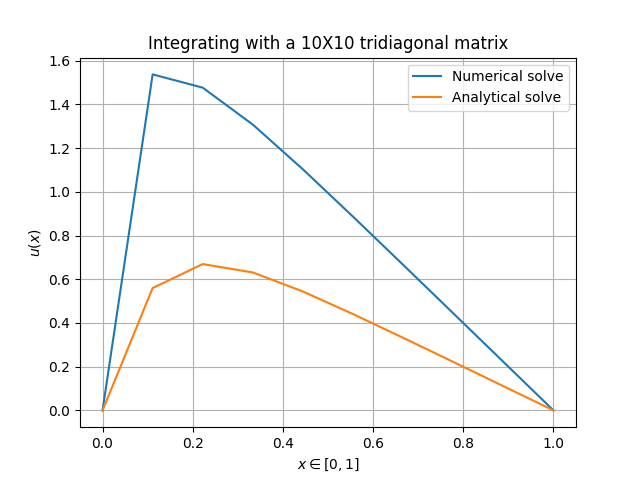
\includegraphics[width=\columnwidth]{../figures/NumVsAnal10x10.png}
	\caption{Plot of numerical, and analytical solution, using the general Thomas algorithm with
	\(N=10\).}
\end{figure}

\begin{figure}[H]
	\centering
	\label{fig:412}
	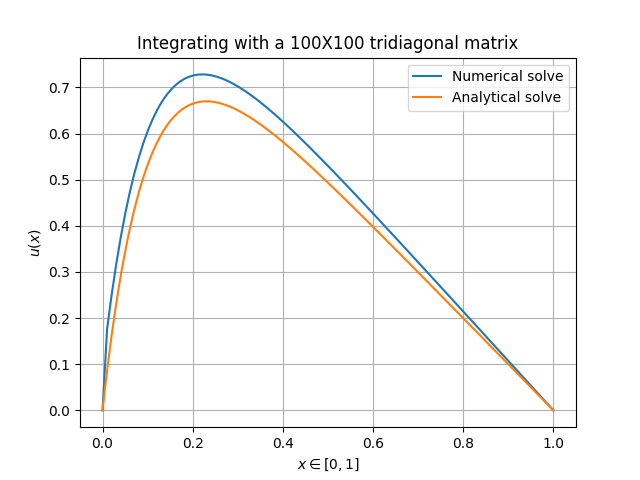
\includegraphics[width=\columnwidth]{../figures/NumVsAnal100x100.png}
	\caption{Plot of numerical, and analytical solution, using the general Thomas algorithm with
	\(N=100\).}
\end{figure}

\begin{figure}[H]
	\centering
	\label{fig:413}
	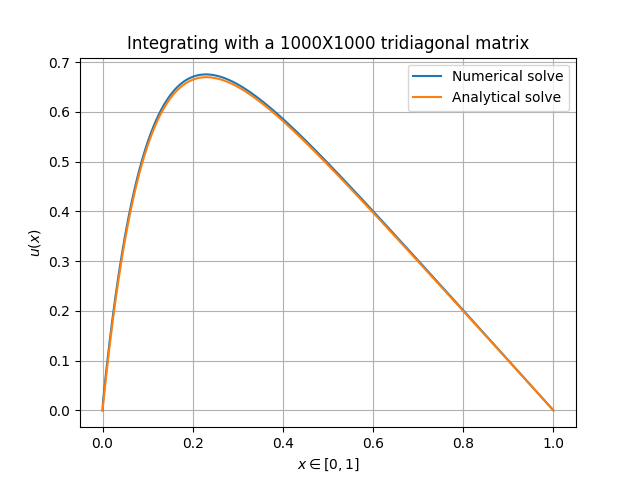
\includegraphics[width=\columnwidth]{../figures/NumVsAnal1000x1000.png}
	\caption{Plot of numerical, and analytical solution, using the general Thomas algorithm with
	\(N=1000\).}
\end{figure}
Using \hyperref[A:1]{"project.py"(A.1)}, I plotted the numerical and analytical solutions to Possion's equation for a spherically symetrical charge distrobution, using a \(N\times N\) matrix. From comparing \hyperref[fig:411]{figure 1} with \hyperref[fig:412]{figure 2}, and \hyperref[fig:413]{figure 3}, I see that the correspondence with the analytical values decreases as the number of matrix elements increases. It was rather unsuprising that a greater \(N\), and therfore smaller step size \(h\), leads to greater accuracy.


\subsection{Benchmarks of the general and specializeed algorithms}\label{subsec:42}
\begin{table}[H]
	\centering
	\label{tab:421}
	\begin{tabular}{l|r}
	\(N\) & Time \([\si{\second}]\) \\
	\(\SI{1e+01}{}\) & \(\SI{3.596200e-04}{}\) \\
	\(\SI{1e+02}{}\) & \(\SI{6.853430e-04}{}\) \\
	\(\SI{1e+03}{}\) & \(\SI{6.667227e-03}{}\) \\
	\(\SI{1e+04}{}\) & \(\SI{6.290169e-02}{}\) \\
	\(\SI{1e+05}{}\) & \(\SI{6.611870e-01}{}\) \\
	\end{tabular}
	\caption{Table of time elapsed in seconds on the general Thomas algorithm for
	\hyperref[A:1]{"project.py"} with corresponding value of \(N\)}
\end{table}

\begin{table}[H]
	\centering
	\label{tab:422}
	\begin{tabular}{l|r}
	\(N\) & Time \([\si{\second}]\) \\
	\(\SI{1e+01}{}\) & \(\SI{4.5119e-05}{}\) \\
	\(\SI{1e+02}{}\) & \(\SI{6.6955e-05}{}\) \\
	\(\SI{1e+03}{}\) & \(\SI{7.45246e-04}{}\) \\
	\(\SI{1e+04}{}\) & \(\SI{7.31116e-03}{}\) \\
	\(\SI{1e+05}{}\) & \(\SI{7.11403e-02}{}\) \\
	\end{tabular}
	\caption{Table of time elapsed in seconds on the specialized Thomas algorithm for
	\hyperref[A:2]{"project\_specialized.py"} with corresponding value of \(N\)}
\end{table}

I mesaured the time both \hyperref[A:1]{"project.py"}, and \hyperref[A:2]{"project\_specialized.py"} used to execute the general and specialized versions of the Thomas algorithm. This was done by saving the time on the CPU-clock directly before and after executing the two sequential loops that constitute the complete algorithm.

\hyperref[tab:421]{Table I} shows the time it took for \hyperref[A:1]{"project.py"}, and \hyperref[tab:422]{table II}
shows the time it took for \hyperref[A:2]{"project\_specialized.py"}. The two afformentioned tables show a decrease in computation time by approximatly one order of magnitude. This was rather suprising given that the number of FLOPs was only halved. However there might be extra overhead associated with retrieving values from arrays that affects the general Thomas algorithm, since it has the elements of the original matrix stored in three arrays, while the specialized Thomas algorithm does not, since any factor containing said elements are precalculated.

There are other possible factors at play, such as seperate processes taking up CPU cycles. Both programs where benchmarked with as few as possible background processes. It was also a posibility that variations in CPU clockspeed might influence the results. A better method of benchmarking would simply have been to take the averages of multiple runs per \(N\)-value.
 
\subsection{Error analysis of the specialized Thomas algorithm}\label{subsec:43}
\begin{table}[H]
	\centering
	\label{tab:431}
	\begin{tabular}{l|r}
	\(\log_{10}h\) & \(\log_{10}\epsilon_{i,max}\) \\
	\(-1\) & \(-0.0176522\) \\
	\(-2\) & \(-0.842497\) \\
	\(-3\) & \(-1.59133\) \\
	\(-4\) & \(-2.41863\) \\
	\(-5\) & \(-3.29336\) \\
	\(-6\) & \(-4.19081\) \\
	\(-7\) & \(-5\) \\
	\end{tabular}
	\caption{Table of \(\log_{10}h\), and the corresponding \(\log_{10}\epsilon_{i,max}\),
	where \(h\) is the step-size used, and \(\epsilon_{i,max}\) is the coresponding
	maximum of the relative error}
\end{table}

To evaluate the accuracy of the specialized Thomas algorithm, I ran \hyperref[A:2]{"project\_specialized.py"} for values of \(N=10^{i}\) where \(i=1,2,...,7\). To compare the numerical and analytical values, I used \hyperref[A:4]{"erroranalysis.py"(A.4)} which reads each data set, and stores a \(7\times 2\)-matrix in a textfile containing the \(\log_{10}\) of the maximum relativ error for each value of \(N\), and the \(log_{10}\) of the coresponding step size. The resulting values in \hyperref[tab:431]{table III} shows that the maximum relativ error of the numerical solution decreases by approximatly one order of magnitude when the step size was decreased by one order of magnitude.

\hyperref[A:4]{"erroranalysis.py"} did output "RuntimeWarning: divide by zero encountered in log10". It was found to happen for \(N=\SI{10e+05}{}\), and by saving and opening the corresponding array of relativ errors, I found that some of the values were \(0\). This does not appear to have affected the resulting maximum error.

\subsection{Comparison with LU-decomposition}\label{subsec:44}
\begin{table}[H]
	\centering
	\label{tab:441}
	\begin{tabular}{l|r}
	\(N\) & Time \([\si{\second}]\) \\
	\(\SI{1e+01}{}\) & \(\SI{2.77714e-04}{}\) \\
	\(\SI{1e+02}{}\) & \(\SI{1.73773e-03}{}\) \\
	\(\SI{1e+03}{}\) & \(\SI{3.07732e-02}{}\) \\
	\(\SI{1e+04}{}\) & \(\SI{6.14422e0}{}\) \\
	\(\SI{1e+05}{}\) & NaN \\
	\end{tabular}
	\caption{Table of time elapsed in seconds on LU decomposition and solve for
	\hyperref[A:2]{"LUdecomp.py"} with corresponding value of \(N\)}
\end{table}
For comparison, I used the LU-decompositon included in the SciPy library. Thdivide by zero in numpy log10e program \hyperref[A:5]{"LUdecomp.py"} which times both the LU factorisation, and solving the resulting system of equations. By comparing  \hyperref[tab:441]{table IV} with \hyperref[tab:421]{table I} and \hyperref[tab:422]{table II}, it becomes apparent that the LU-decompositon was significantly slower.

There was some overhead in the function calls, that \hyperref[A:1]{"project.py"} and \hyperref[A:2]{"project\_specialized.py"} does not have, as they are timed inside their respective functions. However, the more probable reason for the slow down was the increase in FLOPs from \(8N\) and \(4N\) for the general and specialized Thomas-algorithm, to
\(\frac{2}{3}N^{3}\) FLOPs for the LU-decomposition\citep{Hjorth-Jensen2018}, since the LU-decomposition was dealing with all \(N\times N\) elements of the input matrix.

The final entry on \hyperref[tab:441]{table IV} is listed as "not a number" due to \hyperref[A:5]{"LUdecomp.py"} running out of memory and crashing, when atempting to allocate space for all matrix elements when \(N = \SI{1e+05}{}\). This was not suprising, as an \(10^{5}\times 10^{5}\)-matrix where each element is a \(64\)bit floatingpoint number would require \(80\)GB of random access memory. The system I used only had \(16\)GB. By comparison, \hyperref[A:1]{"project.py"} uses only \(2.4\)MB to represent the same matrix, allowing for much greater values of \(N\), and \hyperref[A:2]{"project\_specialized.py"} uses a mere \(800\)kB representing the precalculated \(1/d_{i}^{*}\) factors.

\section{Conclusion}\label{sec:5}
The Thomas algorithm proved to be a efficient, and sufficiently precise method for integrating a second order, linear differential equation. The specialized variant of the algorithm proved especially memory efficient, as discussed in \hyperref[subsec:44]{IV.B}.
Both the general, and specialized Thomas algorithms are preferable for the specific usecase in this paper, as they used significantly less memory, and time than a general LU-decomposition solver.

\bibliography{kilder}{}
\newpage
\appendix
\section{Program files} \label{A}
All code for this report was written in Python 3.6, and the complete set of program files can be found at \url{https://github.com/FunkMarvel/CompPhys-Project-1}.

\subsection{project.py}\label{A:1}
\url{https://github.com/FunkMarvel/CompPhys-Project-1/blob/master/project.py}

\subsection{project\_specialized.py}\label{A:2}
\url{https://github.com/FunkMarvel/CompPhys-Project-1/blob/master/project_specialized.py}

\subsection{data\_generator.py} \label{A:3}
\url{https://github.com/FunkMarvel/CompPhys-Project-1/blob/master/data_generator.py}

\subsection{erroranalysis.py} \label{A:4}
\url{https://github.com/FunkMarvel/CompPhys-Project-1/blob/master/erroranlaysis.py}

\subsection{LUdecomp.py}\label{A:5}
\url{https://github.com/FunkMarvel/CompPhys-Project-1/blob/master/LUdecomp.py}


\end{document}
